\chapter{Metodologia}\label{cap:proposta}

Esta seção descreve a metodologia proposta para a tarefa de classificação da OA de joelho a partir de radiografias. A principal abordagem desta pesquisa consiste no uso de \textit{transfer learning} para aproveitar o conhecimento já obtido por modelos pré-treinados e melhorar a performance da predição final.

\section{Coleta de dados}

A escolha e coleta dos dados é a primeira tarefa a ser realizada quando o objetivo é treinar um modelo de aprendizado profundo, incluindo redes neurais artificiais e vision transformers. Um conjunto de dados adequado é essencial para que o modelo tenha uma boa performance e seja útil para se tornar uma ferramenta de suporte no diagnóstico de OA de joelho. O conjunto de dados foi obtido a partir da plataforma Kaggle \cite{dataset-kaggle}, uma fonte amplamente reconhecida por fornecer dados de alta qualidade e de domínio público para estudos acadêmicos e projetos de aprendizado de máquina. O conjunto de dados escolhido é baseado na Osteoarthritis Initiative (OAI), um estudo observacional multicêntrico de dez anos de homens e mulheres, patrocionado pelo National Institutes of Health (NIH), com o objetivo de permitir uma melhor compreensão da prevenção e tratamento da osteoartrite de joelho \cite{oai}. Este conjunto contém radiografias de joelhos, juntamente com suas respectivas classificações de severidade da OA, conforme o sistema de Kellgren/Lawrence. Este dataset foi selecionado por sua relevância na plataforma, fornecendo uma base sólida para o treinamento dos modelos de RNCs e ViTs propostos nesta pesquisa. A \autoref{tabela-dataset} ilustra os detalhes do conjunto de dados.

\begin{table}[htbp]
    \centering
    \begin{tabular}{|c|c|c|}
        \hline
        \textbf{Classe KL} & \textbf{Número de Imagens} & \textbf{Exemplo de Imagem} \\
        \hline
        0 (saudável) & 3857 & 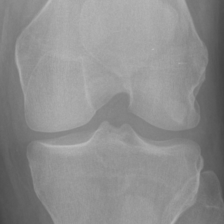
\includegraphics[width=2cm]{figs/KL0-sample.png} \\
        \hline
        1 (duvidoso) & 1770 & 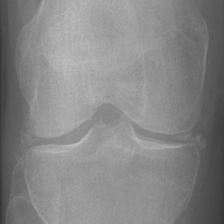
\includegraphics[width=2cm]{figs/KL1-sample.png} \\
        \hline
        2 (mínimo) & 2578 & 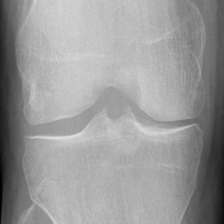
\includegraphics[width=2cm]{figs/KL2-sample.png} \\
        \hline
        3 (moderado) & 1286 & 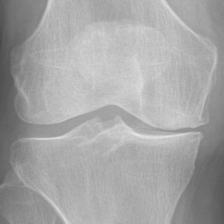
\includegraphics[width=2cm]{figs/KL3-sample.png} \\
        \hline
        4 (severo) & 295 & 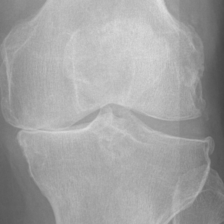
\includegraphics[width=2cm]{figs/KL4-sample.png} \\
        \hline
    \end{tabular}
    \caption{Quantidade de imagens em cada classe Kellgren/Lawrence do conjunto de dados escolhido.}
    \label{tabela-dataset}
\end{table}

O conjunto de dados contém quatro pastas nomeadas ``auto\_test'', ``test'', ``train'' e ``val'', cada uma contendo as subpastas com imagens 224x224 representando cada um dos graus de KL. O dataset foi dividido entre dados de treino, teste e validação, com uma proporção de 7:2:1. O conjunto de treino é usado para treinar os modelos e consiste na maior proporção de imagens. O conjunto de validação é usado para ajustar os hiperparâmetros do modelo e monitorar o seu desempenho, enquanto o conjunto de teste é usado após o treinamento completo do modelo, para medir o desempenho final e verificar sua capacidade de generalização em dados completamente novos.

\section{Pré-processamento das imagens}

O pré-processamento de imagens de raio-X é crucial para melhorar a qualidade e facilitar a análise automatizada pelos modelos. Para isso, algumas técnicas devem ser utilizadas, incluindo:

\subsection{Normalização}

A normalização de dados visa ajustar os valores para um intervalo padrão, melhorando a consistência dos dados e a eficiências dos modelos treinados. Para as radiografias, os pixels devem ter seus valores transformados para o intervalo entre 0 e 1.

\subsection{Equalização}

A equalização busca melhorar o contraste e a visibilidade dos detalhes em uma imagem. O objetivo da equalização é redistribuir os níveis de cinza para que todos os valores de intensidade apareçam com uma frequência mais uniforme. Isso é realizado calculando o histograma acumulado da radiografia original e utilizando-o para redistribuir os valores de pixel.

\subsection{Filtragem e suavização}

As técnicas de filtragem e suavização visam reduzir o ruído e melhorar a qualidade visual das imagens. Para isso, será utilizado o filtro gaussiano, onde cada pixel tem o seu valor substituído pelo valor ponderado da média dos pixels vizinhos, onde os pesos são determinados pela função gaussiana.

\subsection{Aumento de dados}

A ideia desta técnica é expandir artificialmente o tamanho e a variabilidade de um conjunto de dados, principalmente quando o volume de dados disponível é limitado. Isso torna os modelos mais robustos e genéricos, prevenindo \textit{overfitting} e melhorar o desempenho em dados novos. As técnicas de aumento de dados que serão utilizadas nas radiografias são: rotação, escalonamento e reflexão (espelhamento) horizontal.

\section{Arquitetura do modelo de Rede Neural Convolucional}

As redes neurais convolucionais possuem um papel muito relevante no contexto de inteligência artificial, especialmente em tarefas de visão computacional devido à sua capacidade de extrair características relevantes de imagens de forma automática, sem qualquer intervenção manual. Sua arquitetura é especialmente eficaz para reconhecer e classificar objetos em imagens complexas, inclusive em radiografias, com o intuito de auxiliar no processo de diagnóstico médico. As RNCs conseguem identificar variações sutis que podem estar associadas a condições patológicas, como é o caso da osteoartrite de joelho, onde as variações entre os graus de KL reside no espaçamento articular da junção do joelho.

Fazer o treinamento de uma RNC sem nenhum conhecimento prévio do modelo é custoso em termos de quantidade de dados necessário, consumo de recursos computacionais e tempo. Para resolver este problema, o uso de \textit{transfer learning} é essencial, pois permite aproveitar modelos já treinados em grandes conjuntos de dados genéricos, como o ImageNet, e adaptá-los para o conjunto de dados específico para o problema. Ao utilizar o \textit{transfer learning}, as primeiras camadas do modelo, que capturam características gerais da imagem, são congeladas, enquanto as camadas finais são ajustadas para a tarefa específica, tal processo é chamado de \textit{fine-tuning}. Isso economiza tempo e recursos computacionais e aumenta a eficácia do treinamento, resultando em modelos que podem fornecer diagnósticos precisos mesmo com volumes menores de dados disponíveis. Nos últimos anos, algumas arquiteturas performaram muito bem em algumas tarefas, como por exemplo a ResNet, VGG, Inception (GoogLeNet) e DenseNet. A arquitetura para os modelos de RNC pode ser vista na Figura \ref{modelo rnc}.

\subsection{ResNet (Residual Network)}

A ResNet \cite{He2016} é uma arquitetura amplamente utilizada em tarefas de classificação de imagens devido à sua capacidade de treinar redes profundas sem problemas de desaparecimento de gradiente. A inovação da ResNet está em seus blocos residuais, que introduzem conexões de atalho para permitir que os gradientes fluam melhor durante o treinamento. Isso torna a ResNet altamente eficiente para tarefas de classificação de imagens médicas. Para este trabalho, serão treinados os modelos ResNet34, ResNet50 e ResNet101, que oferecem um bom equilíbrio entre profundidade e performance.

\subsection{VGG (Visual Geometry Group Network)}

O VGG \cite{Simonyan2015} é um modelo mais simples comparado ao ResNet, mas ainda é muito eficaz. Ele se destaca por usar camadas convolucionais de pequenos filtros (3x3) empilhadas seguidas por camadas de pooling. Embora o VGG tenha mais parâmetros que modelos mais modernos, sua estrutura é eficaz para capturar detalhes visuais em imagens médicas. O VGG16 e VGG19 serão utilizados nesta pesquisa.

\subsection{DenseNet (Densely Connected Convolutional Networks)}

O DenseNet \cite{Huang2017} utiliza conexões densamente conectadas, onde cada camada recebe entradas de todas as camadas anteriores. Isso promove um fluxo eficiente de gradientes e incentiva o reuso de características aprendidas, o que pode ser muito útil nas radiografias de osteoartrite de joelho, onde detalhes finos precisam ser capturados, especialmente na diferenciação entre graus de KL adjacentes. Os modelos do DenseNet121 e DenseNet169 serão as opções para este trabalho.

\subsection{Inception (GoogLeNet)}

A rede Inception \cite{Szegedy2016}, também chamada de GoogLeNet, é conhecida por seu uso de módulos Inception, que permitem que a rede aprenda de forma mais eficiente ao explorar convoluções de diferentes tamanhos em paralelo. A habilidade da Inception de capturar informações em várias escalas pode ser especialmente útil ao lidar com imagens médicas de diferentes resoluções. O Inception-v3 é uma versão mais moderna e, portanto, será utilizada nesta pesquisa.

\begin{figure}[h]
    \centering
    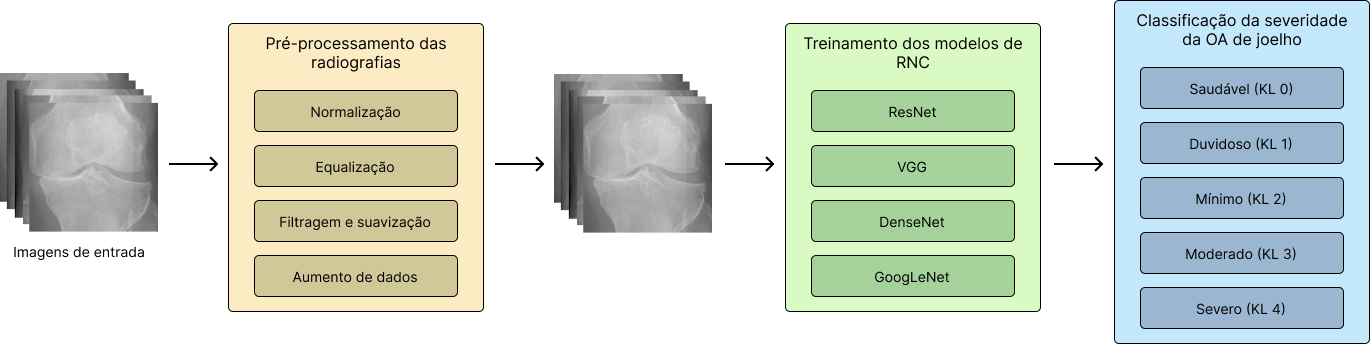
\includegraphics[width=\linewidth]{figs/modelo-rnc.png}
    \caption{Metodologia para as redes neurais convolucionais}
    \label{modelo rnc}
\end{figure}

\section{Arquitetura do modelo de Vision Transformer}

A arquitetura Vision Transformer tem se detacado como uma abordagem poderosa para tarefas de visão computacional devido à sua capacidade de capturar relações globais em imagens através do mecanismo de atenção \cite{Dosovitskiy2021}. Essa abordagem permite que os modelos de ViTs alcancem ótimos resultados e superem as limitações das RNCs, que focam mais em características locais da imagem. Tal capacidade é particularmente relevante para o diagnóstico de patologias em imagens médicas, incluindo radiografias, onde o modelo é capaz de processar toda a imagem simultaneamente, associando partes distantes e próximas com igual relevância. Além disso, os ViTs também se beneficiam do \textit{transfer learning}, permitindo que os modelos sejam treinados de forma eficiente em conjuntos de dados limitados. Para esta pesquisa será feito o \textit{fine-tuning} de alguns modelos de ViT para a tarefa de classificação da OA de joelho, como o ViT-B/16, DeiT (Data-efficient Image Transformer), Swin Transformer (Shifted Window Transformer) e ResNet50-ViT-B/16. A arquitetura para os modelos de ViT pode ser vista na Figura \ref{modelo vit}.

\subsection{ViT-B/16}

O ViT-B/16 \cite{Dosovitskiy2021} é uma das primeiras variantes da arquitetura Vision Transformer, onde "B" representa o modelo base (base model) e "16" refere-se ao tamanho do \textit{patch} em que a imagem é dividida (16x16 pixels). O ViT-B/16 recebe uma imagem e a divide em \textit{patches}, tratando cada \textit{patch} como um \textit{token}, semelhante ao processamento de palavras em texto nos \textit{transformers} tradicionais. O modelo usa um mecanismo de atenção para processar os \textit{tokens} de maneira global, capturando interdependências entre diferentes regiões da radiografia. Essa abordagem permite que o ViT-B/16 compreenda melhor a estrutura geral da imagem, identificando padrões que podem se estender por grandes áreas da mesma. Este modelo pode ser especialmente eficaz para a tarefa de classificação da OA de joelho, visto que existe o padrão notável do espaçamento articular que se extende horizontalmente na radiografia.

\subsection{DeiT (Data-efficient Image Transformer)}

O DeiT \cite{Touvron2021} é uma versão otimizada dos ViTs, projetada para melhorar a eficiência no uso de dados. Enquanto os ViTs originais, como o ViT-B/16, geralmente precisam de grandes quantidades de dados para atingir um bom desempenho, o DeiT foi projetado para ser treinado em conjunto de dados reduzidos. Isso acontece devido à técnica do \textit{ditillation token}, que permite ao modelo aprender a partir de um "professor" (modelo mais simples), aumentando a eficiência do treinamento. Este modelo pode ser particularmente útil na tarefa de classificação da OA de joelho, podendo ser um importante fator ao comparar com outros modelos de ViTs e RNCs.

\subsection{Swin Transformer (Shifted Window Transformer)}

O Swin Transformer \cite{Liu2021} é uma arquitetura de ViT que introduz uma abordagem nova que utiliza \textit{hierarchical feature maps} e \textit{sliding windows} para aplicar a atenção e melhorar a eficiência e performance do modelo. Em vez de processar toda a imagem como uma sequência de \textit{patches} globalmente, o Swin Transformer aplica a atenção dentro de pequenas janelas locais, de forma hierárquica, permitindo que o modelo mantenha a eficiência computacional e ainda capture detalhes locais e globais. Conforme o modelo avança pelas camadas, as janelas se expandem e se deslocam, permitindo que o modelo agregue contexto global ao longo do processamento. Essa estrutura hierárquica é particularmente eficaz para imagens de alta resolução, como as radiografias, onde há muitos detalhes importantes em diferentes escalas. Além disso, o Swin Transformer pode ser facilmente escalado para diferentes tamanhos de imagens e é altamente eficiente em termos de uso de memória e poder computacional, sendo uma escolha apropriada para a tarefa de classificação da OA de joelho.

\subsection{ResNet50-ViT-B/16}

Uma abordagem híbrida, combinando RNC, como o ResNet, e ViT, pode ser aplicada de maneira eficaz na classificação da severidade da osteoartrite de joelho, aproveitando as vantagens de ambas as arquiteturas para obter uma melhor predição das classificações de KL \cite{Park2022, Wang2021}. Essa mescla pode ser observada no modelo ResNet50-ViT-B/16, onde o ResNet50 atua como um extrator de características iniciais, processando as radiografias e capturando padrões como texturas e bordas, e o modelo ViT-B/16 utiliza seus mecanismos de atenção para permitir uma análise mais contextualizada e eficiente. A combinação se faz promissora para melhorar a precisão na classificação da OA de joelho, equilibrando eficiência computacional e qualidade do modelo final.

\begin{figure}[h]
    \centering
    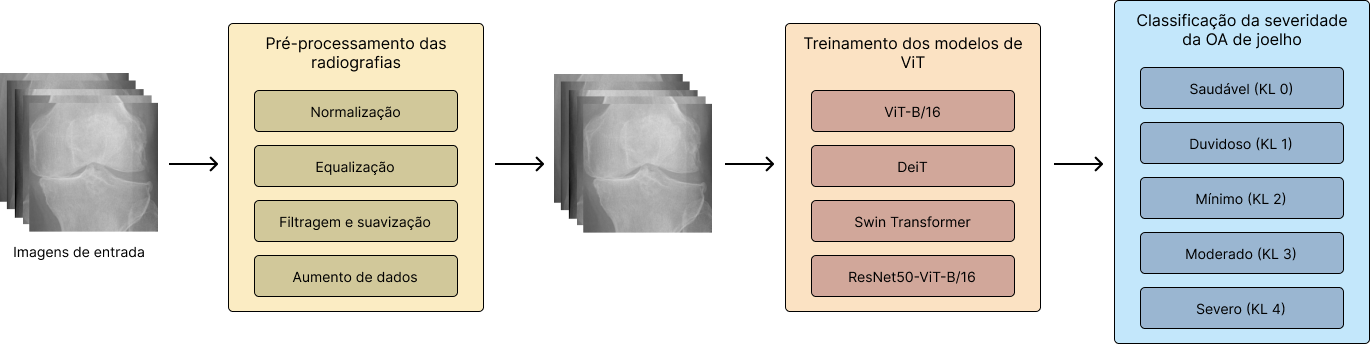
\includegraphics[width=\linewidth]{figs/modelo-vit.png}
    \caption{Metodologia para os vision transformers}
    \label{modelo vit}
\end{figure}

\section{Métricas de avaliação}

Para comparar a performance dos modelos treinados na tarefa de classificação da severidade da OA de joelho, serão utilizadas as seguintes métricas de avaliação: acurácia, precisão, revocação, F1-score e matriz de confusão. Essas métricas são amplamente utilizadas em problemas de classificação para medir a qualidade das previsões e o equilíbrio entre os diferentes tipos de erros. Para o cálculo das métricas, os seguintes acrônimos serão utilizados nas fórmulas:

\begin{itemize}
    \item $TP$ é o número de verdadeiros positivos,
    \item $TN$ é o número de verdadeiros negativos,
    \item $FP$ é o número de falsos positivos,
    \item $FN$ é o número de falsos negativos.
\end{itemize}

\subsection{Acurácia}
A acurácia mede a proporção de previsões corretas em relação ao total de exemplos. Ela pode ser calculada pela fórmula:

\begin{equation}
    \text{Acurácia} = \frac{TP + TN}{TP + TN + FP + FN}
\end{equation}

\subsection{Precisão}
A precisão indica a proporção de exemplos classificados como positivos que realmente são positivos. Ela é calculada pela fórmula:

\begin{equation}
    \text{Precisão} = \frac{TP}{TP + FP}
\end{equation}

\subsection{Recall}
O recall mede a capacidade do modelo de identificar corretamente todos os exemplos positivos. É definido como:

\begin{equation}
    \text{Recall} = \frac{TP}{TP + FN}
\end{equation}

\subsection{F1-Score}
O F1-score é a média harmônica entre precisão e recall, e é uma métrica útil quando busca-se um equilíbrio entre os dois. A fórmula do F1-score é:

\begin{equation}
    F1 = 2 \cdot \frac{\text{Precisão} \cdot \text{Recall}}{\text{Precisão} + \text{Recall}}
\end{equation}

\subsection{Matriz de Confusão}
A matriz de confusão é uma ferramenta para visualizar o desempenho do modelo de classificação, detalhando as previsões corretas e incorretas em cada classe. Ela apresenta os valores de $TP$, $TN$, $FP$ e $FN$ de forma estruturada, permitindo avaliar o desempenho em classes específicas.

\[
\begin{array}{|c|c|c|}
\hline
 & \text{Previsto Positivo} & \text{Previsto Negativo} \\
\hline
\text{Verdadeiro Positivo} & TP & FN \\
\hline
\text{Verdadeiro Negativo} & FP & TN \\
\hline
\end{array}
\]

\subsection{AUC-ROC}
Para tarefas de classificação binária, será utilizada também a métrica AUC-ROC (Área Sob a Curva da Característica de Operação do Receptor), que mede a capacidade do modelo de separar as classes positivas e negativas. A curva ROC é um gráfico que exibe a taxa de verdadeiros positivos (sensibilidade) em função da taxa de falsos positivos.

\begin{equation}
    \text{AUC-ROC} = \int_{0}^{1} \text{TPR}(FPR) dFPR
\end{equation}

onde $TPR$ é a taxa de verdadeiros positivos e $FPR$ é a taxa de falsos positivos.

\section{Método de visualização}

A visualização é uma técnica importante para avaliar quais foram as regiões da imagens que ajudaram o modelo a fazer determinada previsão. O método de visualização Grad-CAM (Gradient-weighted Class Activation Mapping) é uma técnica usada para interpretar e visualizar as decisões feitas por redes neurais convolucionais (RNCs). Em tarefas de classificação, como a avaliação da severidade da OA de joelho a partir de radiografias, entender quais regiões da imagem contribuíram para a decisão do modelo é crucial para a validação e a confiança nos resultados do modelo.

O Grad-CAM fornece mapas de ativação que mostram quais partes da imagem foram mais influentes para a predição de uma classe específica \cite{Selvaraju2016}. Para isso, essa técnica utiliza os gradientes da saída da camada final da rede em relação às ativações das camadas intermediárias para gerar uma visualização da importância das regiões da imagem.

Primeiro, é gerado um mapa de localização a partir da RNC utilizada para classificar a imagem usando a técnica do Class Activation Mapping (CAM). O CAM utiliza mapas de características convolucionais, que são globalmente agrupados usando a técnica de \textit{Global Average Pooling} (GAP) e transformados linearmente para produzir uma pontuação \( y_c \) para cada classe \( c \). Especificamente, se a penúltima camada da RNC produz \( K \) mapas de características \( A_k \in \mathbb{R}^{u \times v} \), esses mapas são agrupados espacialmente e combinados linearmente para gerar a pontuação:

\[
y_c = \sum_k w_{ck} \frac{1}{Z} \sum_i \sum_j A_{k_{ij}}
\]

Para produzir o mapa de localização \( L_c^{CAM} \) para a classe \( c \), CAM calcula a combinação linear dos mapas de características finais usando os pesos aprendidos da camada final:

\[
L_c^{CAM} = \sum_k w_{ck} A_k
\]

Este mapa é então normalizado para o intervalo entre 0 e 1 para fins de visualização.

Em seguida, os gradientes são então globalmente averiguados (\textit{pooling}) para obter pesos que indicam a importância de cada canal de ativação. Esses pesos são usados para ponderar as ativações da camada convolucional final. A seguinte fórmula representa este cálculo dos pesos:

\[
\alpha_{k}^{c} = \frac{1}{Z} \sum_i \sum_j \frac{\partial y^{c}}{\partial A_{ij}^{k}}
\]

O peso \( \alpha_{k}^{c} \) representa a linearização parcial da rede e captura a importância de \(k \) para a classe \(c \). Por fim, o mapa de ativação é obtido ao multiplicar as ativações ponderadas pelos pesos dos gradientes. Esse mapa é então normalizado e sobreposto na imagem original para mostrar as áreas mais influentes na decisão do modelo.

A fórmula para o Grad-CAM pode ser expressa como:

\[
\text{Grad-CAM} = \text{ReLU} \left( \sum_{k} \alpha_{k}^{c} A^{k} \right)
\]

Para esta pesquisa, a utilização do Grad-CAM permitirá a visualização das regiões das radiografias que o modelo considera mais relevantes para suas decisões de classificação. Isso não só facilita a interpretação dos resultados do modelo, mas também ajuda na validação de sua eficácia ao garantir que o modelo está focando nas áreas corretas da imagem, como o espaço articular do joelho.